


% This LaTeX was auto-generated from an M-file by MATLAB.
% To make changes, update the M-file and republish this document.






  
    

\section{Example 6 - Further Study} \label{sec:Ex6Tests}
This script file tests the slope problem from example 6, which has been
seen to create spurious results for the GenAlg module. The slope problem
will be given a consistency test to investigate the performance issues.

\subsection{Testing}
The genetic algorithm search is performed 10 times. The results of each
critical slip are plotted in the following figure. The figure shows
little difference between the slips that converge to factor of safety of
1 and those that converge below, other than the sharp incline the low
factor of safety slopes show at the slip exit.


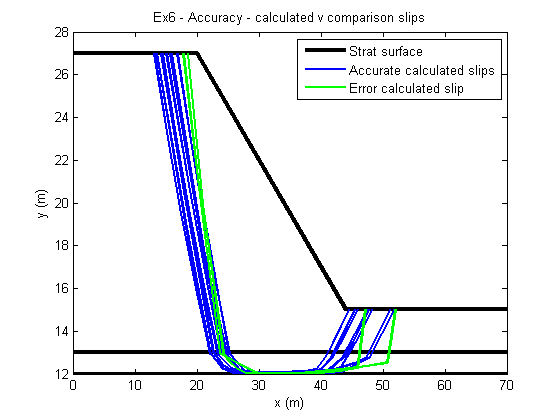
\includegraphics [width=5in]{./VV_SubDocuments/SSA_Ex6Tester_01.png}



The next figure shows the progression of the factors of safety through
the generations for each search. The results tend to not show a single
specific path the slips with factors of safety less than 1 take towards
convergence.


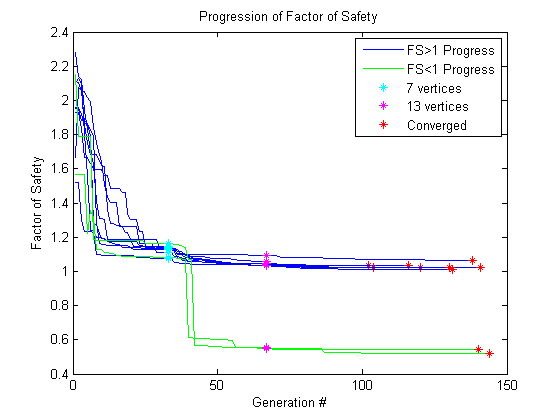
\includegraphics [width=5in]{./VV_SubDocuments/SSA_Ex6Tester_02.png}



The next figure of the distribution of factors of safety clearly shows
the bimodal distribution of critical factors of safety generated by the
search.


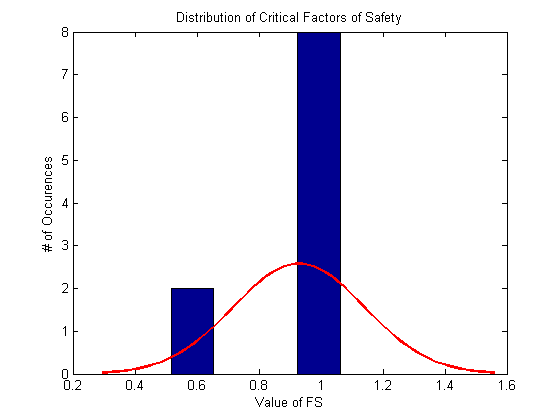
\includegraphics [width=5in]{./VV_SubDocuments/SSA_Ex6Tester_03.png}



The genetic algorithm operates by using the Morgenstern Price algorithm
to calculate factors of safety. The factor of safety calculated for the
critical slip by the Morgenstern Price solver is compared to the Rigid
finite element algorithm. Results found in the following table.

        
\color{lightgray} \begin{verbatim}
Type       Morgenstern Price        RFEM    relative error
Accurate        1.0217            1.1683      14.3456
Accurate        1.0345            1.2078      16.7444
Accurate        1.0617            1.1922      12.2930
Accurate        1.0205            1.1641      14.0712
Accurate        1.0353            1.1929      15.2284
Accurate        1.0209            1.1672      14.3306
Accurate        1.0097            1.1520      14.0884
Accurate        1.0248            1.1572      12.9240
Error           0.5428            1.3583      150.2475
Error           0.5173            1.3861      167.9533

\end{verbatim} \color{black}
    

These results show disagreement between the Morgenstern Price and RFEM
algorithms, specifically towards the slip surfaces that produce factors
of safety less than 1 in the Morgenstern Price algorithm. This could
suggest that slip surfaces in with the sharp angles shape seen are
difficult for the Morgenstern Price algorithm to calculate accurately.

Next the sharp angle seen produced by the failure cases is studied by
measuring the angle of the final rise of the slip surfaces. Results in
the table below show that the $FS < 1$ cases have a significantly sharper
exit angle. This continues to suggest that the shape of the failure slips
may be the performance issues.

        
\color{lightgray} \begin{verbatim}
Type        exit angle        Kin Pass    Failure Code
Accurate        2.5570               1          
Accurate        2.4633               1          
Accurate        2.3903               1          
Accurate        2.6349               1          
Accurate        2.4936               1          
Accurate        2.5700               1          
Accurate        2.5328               1          
Accurate        2.4775               1          
Error           2.1022               1           
Error           2.0672               1           

The average rise angle of the slopes with factors of safety
 greater than 1 is 2.515 rads, while the average rise angle 
 of slopes with factors of safety less than 1 is 2.085 rads.
\end{verbatim} \color{black}
    

Using a special test case, where the minimum allowable angle was raised
(to 2.3 rads, 130 deg) the occurrence rate of low factor of safety 
results produced by the genetic algorithm is seen to drop. This could be 
a case that the shape of the failure surface is the performance issue, 
but may also simply be masking a different performance issue. This change
produced no noticeable affect on the results of the other genetic
algorithm calculations performed in \ref{sec:GenAlgTests}. A case could
be made for raising the minimum allowable angle, but a wider range of
test cases would have to be studied before making this decision.
